\documentclass{svproc}
\usepackage{graphicx} 
\usepackage{amsmath}
\usepackage[sorting=none,style=numeric]{biblatex}
\usepackage{soul} %for highlighting
\usepackage{xcolor} %for highlighting
\usepackage{hyperref} %for hyperlink
\usepackage{pdfpages} % for coversheet
\addbibresource{lit.bib}

\title{Exploring a Small Vision Language Model Approach for Vision and Language Navigation Tasks in Continuous Environments}
\author{Wesley Chiu, Abdulrahman Altahhan}
\institute{University of Leeds, School of Computing, ODL MSc in AI, UK. \\ \texttt{\{od22wc, a.altahhan\}@leeds.ac.uk}}
\date{January 2025}
\begin{document}

\includepdf[pages=1]{/home/wes/Documents/git_ws/OCOM5300M_ResearchProject/report/OCOM5300M_coversheet.pdf}
\maketitle

\begin{abstract}
    Vision and Language Navigation (VLN) is a rapidly evolving field of research that aims to enable an embodied agent to follow textual instructions given in natural language to navigate through an unseen environment to a goal position. Existing approaches to this task all into two main categories: "textual" models that aim to tackle the challenge of multi-modality in the textual space, and "integrated" approaches that integrate vision and language models in the latent space. Regardless of the approach, prior work in the field have typically used the largest and most powerful variants of Large Language Models and Vision Models available (70B+ parameters). This work aims to evaluate the suitability of using a lighter-weight variant of an existing open-sourced model  as the primary VLM, which would allow it to be run "on-device" rather than outsourcing its inferencing to a networked compute. The experiments in a simulated environment demonstrates that the current ability of the lighter-weight model is not yet fit for purpose, failing to reach the success rates seen in approaches that use the full-sized variants.
    \\
    Code is available at: \href{https://github.com/wsychiu/OCOM5300M\_ResearchProject}{github.com/wsychiu/OCOM5300M\_ResearchProject}
    
    \keywords{Vision-and-Language Navigation, Vision Language Model, Large Language Model, Prompting}
\end{abstract}

\section{Introduction}
    Vision and Language Navigation (VLN) tasks, which tasks an embodied agent to follow a set of textual instructions given in natural language to navigate a previously unseen 3D indoor environment, have received increasing attention in recent years. Whilst initial research leveraged models such as RNNs and CNNs to process natural language and vision data, the introduction of Transformer-based models \cite{attenion_is_all_you_need} has accelerated capabilities in Natural Language Processing (NLP) and Computer Vision (CV) - both key components in the VLN task. The rapid development of Large Language Models (LLMs) and Vision-Language Models (VLMs) has further intensified the volume and pace of research in VLN, with each advance in LLM and VLM competency benefiting the VLN task.
    The original VLN task, as proposed by Andersen, et al. \cite{mattersim}, requires the agent to navigate between pre-defined nodes in the environment (referred to as a navigation graph), which essentially reduces the VLN task to a vision-based graph-search problem; models trained in this manner have difficulty translating performance to real-world environments \cite{pmlr-v155-anderson21a}. To help combat this gap, the VLN Continuous Environment (VLN-CE) task was introduced, and has no such predefined navigation points, requiring agents to take low-level actions to reach a navigable point in the environment. This introduces new challenges for the models to overcome, such as avoiding getting stuck on obstacles and dealing with distances \cite{krantz2020navgraphvisionandlanguagenavigationcontinuous}.
    \\ \\
    Approaches to the VLN task (whether graph-based VLN or VLN-CE) that leverage existing LLMs and VLMs typically fall into two broad categories: "textual" models or "integrated" models. Textual models \cite{long2023_discussnav, pan2024langnavlanguageperceptualrepresentation, zhou2023navgptexplicitreasoningvisionandlanguage, lin2024navcotboostingllmbasedvisionandlanguage, open-nav} typically use an LLM, such as OpenAI's ChatGPT \cite{openai2024gpt4technicalreport}, with a vision model or image captioning model, such as BLIP \cite{li2022blipbootstrappinglanguageimagepretraining}, by 'connecting' the two models through text. The vision model will generate a textual description of the agent's observations before sending this description to the LLM. Whilst such approaches are able to interface between the two models without extensive training or finetuning, the richness of image data may be lost as it becomes summarised in textual form \cite{pan2024langnavlanguageperceptualrepresentation}. Integrated models \cite{hong2021_vlnbert, navgpt2, chen2021_HAMT, HE2024110511_MemoryAdaptiveVLN} connect the vision and language model(s) in the latent space. These approaches have exhibited stronger performance in VLN tasks compared to the textual model approach (at the time of their release), but are less unable to take advantage of more competent LLMs or VLMs as they are released in the same 'plug-and-play' manner of textual models. This is due to the extensive training and finetuning the integrated architecture requires.
    \\ \\
    The development of Vision Language Models (VLMs) pretrained on a variety of tasks and with strong multi-modal performance \cite{Qwen-VL, Qwen2VL, qwen2, geminiteam2024geminifamilyhighlycapable, openai2024gpt4technicalreport} suggests that an alternative method that strikes a balance between the two approaches could be viable. Additionally, most prior work typically leverage larger, complex language and vision models, often with parameter counts in the tens of billions, requiring powerful hardware to support during inferencing. The development of Low Rank Adaptation (LoRA) finetuning \cite{LoRA} combined with model quantization \cite{MLSYS2024_42a452cb} allows for a LLM or VLM to be trained and run on hardware with more limited memory. This is particularly relevant to the VLN task, as lighter-weight models can be run more readily on smaller robots with more limited hardware, broadening the application of these models.
    \\ \\
    This work proposes, as its main contribution, to explore the effectiveness of using a small, finetuned, quantized open-sourced model as the primary VLM (specifically, Qwen2-VL-7B) to tackle the VLN-CE task and examines its performance against other approaches. 

\section{Literature Review}
    \textbf{Vision and Language Navigation (VLN)}  The ability for an embodied agent to navigate a previously unseen environment purely by natural language instruction is a field of research that has seen increasing interest since the task was formally introduced by Andersen et al. \cite{8578485}. The VLN task requires that an embodied agent be able to navigate an unstructured and previously unseen environment by following navigation instructions provided in natural language. Early research focused on the use of Recurrent Neural Networks (RNNs) \cite{8578485, 8954045, 8953608, li2019robustnavigationlanguagepretraining}; however, with the introduction of the Transformer archicture \cite{attenion_is_all_you_need} and the subsequent development of the Large Language Model (LLM) \cite{radford2018improving, touvron2023llamaopenefficientfoundation}, recent research has focused on leveraging the NLP capabilities of LLMs; these approaches can be broadly categorised into two different approaches: a text-based approach and an integrated approach.
    \\ \\
    \textbf{Textual vs Integrated Approaches} The text-based approach seeks to address the challenge of multi-modality by translating visual features from the agent's observations into textual space. LangNav \cite{pan2024langnavlanguageperceptualrepresentation} and NavGPT \cite{zhou2023navgptexplicitreasoningvisionandlanguage}, for example, used image captioning models such as BLIP \cite{li2022blipbootstrappinglanguageimagepretraining, li2023blip2bootstrappinglanguageimagepretraining} and DETR \cite{zhu2021deformabledetrdeformabletransformers} to caption images and identify objects in those images; this textual information was then passed to GPT-4 for decision making and other navigation tasks; OpenNav \cite{open-nav} takes a similar approach with open-sourced models. Variations on this approach include DiscussNav \cite{long2023_discussnav}, which uses a similar mechanism to enable discussions between its multiple domain experts, as well as NavCoT \cite{lin2024navcotboostingllmbasedvisionandlanguage}, which asks the LLM to predict information about observations from future states and structures its reasonings via chain-of-thought prompting. Integrated approaches also leverage LLMs and image captioning or vision transformer models \cite{dosovitskiy2021imageworth16x16words}, but integrates both models in the latent space through pre-training. These models are typically more performant than the text-based approaches, as the richness of the image data remains captured and transferred between the vision and language models \cite{pan2024langnavlanguageperceptualrepresentation}. Early works in VLN typically required the fusion of text and image encoding via pretraining, such as PREVALENT \cite{9156554}, the CMA model \cite{krantz2020navgraphvisionandlanguagenavigationcontinuous}, and Airbert \cite{Guhur_2021_ICCV}. Recent models build on this work and also grow in complexity as researchers work to capture more proficiency in the VLN task. HAMT \cite{chen2021_HAMT} combined BERT \cite{devlin-etal-2019-bert} encodings with a custom-trained Vision Transformer \cite{dosovitskiy2021imageworth16x16words} and a form of spatial-temporal encoding.  Nav-GPT2 \cite{navgpt2} integrates LLMs with InstructBLIP \cite{dai2023instructblipgeneralpurposevisionlanguagemodels}, a VLM, via a vision encoder \cite{10203681}. In a slightly different approach, SayCan \cite{51647} connects an LLM with a model trained via Reinforcement Learning to robotic affordance. These models, at time of release, were all State of the Art (SOTA), and continue to be referenced as benchmarks against new approaches; however, to obtain such proficiency, extensive pretraining and finetuning is required.
    \\ \\
    \textbf{Specialist Modules}  Independent of the approach, VLN models typically contain multiple "modules" that specialise in particular tasks \cite{wu2022visionlanguagenavigationsurveytaxonomy}; these are either separate models or different types of prompts fed to a single model. Common modules include the action-decision (or policy) module, progress monitor module, and a navigation history module. LangNav \cite{pan2024langnavlanguageperceptualrepresentation}, for example, uses LLaMA2-7B to both select the action and update historical trajectory by using different prompt templates. NavGPT \cite{zhou2023navgptexplicitreasoningvisionandlanguage} takes a similar approach by using a Prompt Manager module with GPT-4 to dynamically change the prompt in response to changes in the agent's state. Some approaches \cite{chen2021_HAMT, HE2024110511_MemoryAdaptiveVLN} have improved progress monitoring by creating specialist architectures to enhance the usefulness of the historical trajectory, whilst other work \cite{9879544, chen-etal-2024-mapgpt} seeks to retain historical trajectory as a graph.
    \\ \\
    \textbf{Vision Language Models}  Early research in VLN required researchers to tackle the task of multi-modal input by integrating separately trained language and vision models. Further research in multi-modal models have developed more tightly integrated foundation models such as InstructBLIP \cite{dai2023instructblipgeneralpurposevisionlanguagemodels}, which allow researchers to finetune a pretrained multi-modal model. More recent research has expanded the competency of multi-modal foundation models, with notable closed-sourced models such as OpenAI's GPT4-V \cite{openai2024gpt4technicalreport} and o1 \cite{openai_o1} models, as well as Google's Gemini \cite{geminiteam2024geminifamilyhighlycapable}, whilst open-sourced models, such as LLaVa \cite{liu2023visualinstructiontuning} and Qwen2-VL \cite{Qwen2VL}, provide a lower-cost and more flexible alternative. Qwen2-VL, in particular, has released three variants of its VLM, with the full model containing 72B parameters, whilst the smallest contains just 2B; the 7B parameter variant, however, aims to strike a balance between model size and performance \cite{vlm_leaderboard}.
    \\ \\
    \textbf{Challenges in Continuous Environments}  A key challenge for VLN agents trained with graph-style navigation ("high-level actions") is the ability to transfer the learning into a real world environment; Andersen et al. \cite{anderson2020simtorealtransfervisionandlanguagenavigation} note a degradation in performance due to these factors. There have been some efforts to translate models trained in navigation-graph based VLN (also referred to as discrete VLN) to continuous environment, but a performance gap remains \cite{Hong_2022_CVPR}. Continuous environments remove the implicit assumptions in navigation-graph style environments, requiring agents to consider new challenges such as environment topology and imperfect localisation in their decision-making process to select the next best "low-level action" to take \cite{krantz2020navgraphvisionandlanguagenavigationcontinuous}. To address these challenges, the originally proposed navigation-graph based Matterport3D Simulator \cite{mattersim} is now eschewed in VLN research in favour of the Habitat-Sim simulator \cite{habitat19iccv, szot2021habitat, puig2023habitat3}, a continuous environment simular.

\section{Methodology}
    \begin{figure}
        \centering
        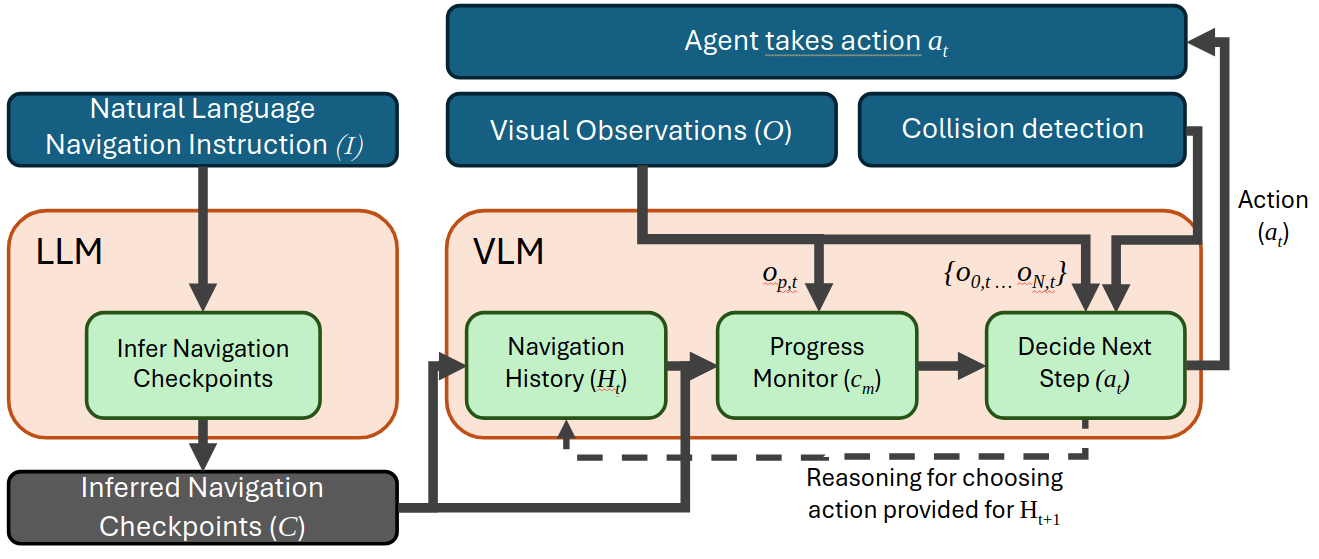
\includegraphics[scale=.28]{figures/OCOM5300M_VLN_Model.png}
        \caption{The architecture of the model used in this work. The LLM is used only to create a structured list of Navigation Checkpoints that also act as sub-goals or medium-term goals for the agent to progress toward, and is useful for orienting the agent in instances where the final goal location may not be visible as well as for monitoring progress. The VLM, with its multi-modal capabilities, is used for all other tasks. Unlike prior work, with its pretrained vision and language capabilities, the VLM negates the requirement to run separate models for image captioning and reasoning tasks.}
        \label{fig:fig1}
    \end{figure}
    The approach taken in this work, as illustrated in Figure \ref{fig:fig1}, comprises of using a single VLM as the primary component of the model to enable the model to determine its current location in the environment, track its historical trajectory, and to make decisions on its next action. A small component of this architecture leverages an LLM to break down the natural language instructions into discrete "Navigation Checkpoints", which is in line with prior work \cite{ chen-etal-2024-mapgpt, pan2024langnavlanguageperceptualrepresentation, zhou2023navgptexplicitreasoningvisionandlanguage}.
    
\subsection{Problem Formulation}
    The VLN-CE task asks an embodied agent to autonomously navigate from a specified starting point to a goal location in an unseen environment by following a path described by natural language instructions. That is, given a natural language navigation instruction $\mathcal{I}$ and a starting state $s_0$, at each step $t$ the agent must determine its current location in the environment and its current progress to take an action $a_t$ that will lead it closer to the goal state $s_G$. The agent observes its environment through sensor observations $O_t$. In this work, $O_t$ is comprised of colour images from $N$ different views, each set at a different angle from the egocentric perspective of the agent. Additionally, the agent is also able to observe the environment through an egocentric panoramic image $o_{p,t}$. That is, the observations at each step is represented by $O_t = \{o_{p,t}, o_{0, t}, ..., o_{N,t}\}$. At each step, the agent must choose to take an action which corresponds to an image direction (excluding $o_{p,t}$), i.e. $a_t \in \{o_{0,t}, ..., o_{N,t}\}$, unless a specific direction is determined to result in a collision with the environment, in which case that particular direction is removed from the action set. The agent is deemed to have successfully reached $s_G$ if the final state of the agent $s_T$, where $T$ is the total number of steps taken, is within 3.0 metres of $s_G$.

\subsection{Framework and Prompts}
    Unlike prior work that used separate Vision and Language models \cite{zhou2023navgptexplicitreasoningvisionandlanguage, 51647} which require pre-training to combine the different models, this work proposes the use of a singular VLM to manage both the image and textual inputs. The VLM is used for three different purposes: to track Navigation History, Decide the Next Navigation Checkpoint to work toward, and to Decide the Next Step. Only one task, creating Inferred Navigation Checkpoints, is not given to the VLM, and is instead given to the LLM. 
    \\ \\
    \textbf{Inferred Navigation Checkpoints}  The navigation instructions is given in natural language, and can include discourse markers that may not be relevant to the navigation itself (e.g. \texttt{"Okay, now ..."}) and may be confusing or difficult to track progress against. To address this, this work follows prior work \cite{open-nav,navgpt2} and uses an LLM to convert $\mathcal{I}$ into a list of Navigation Checkpoints ($C$), which is easier for the model to track progress against. That is, for each $\mathcal{I}$, a series of $M$ Navigation Checkpoints $C = \{C_0, ..., C_M\}$ are created such that by progressing from $c_0$ (the starting point of the instruction) to $c_M$ will result in a successful trajectory (i.e. $s_T \leq s_G\pm 3.0 \text{ metres}$). This can be represented as:
    \\ \\
    \textbf{Navigation History}  A key component to the success of VLN agents is that at the time of deciding the optimal $a_{t+1}$ the agent has the capability to retain in its context a history of its navigational trajectory \cite{chen2021_HAMT, HE2024110511_MemoryAdaptiveVLN}. In this work, at each step, the VLM is prompted to generate $h_t$, which is a summary of the reasoning given for selecting $a_t$ and the agent's current location based on $o_{p,t}$. The VLM is provided with $C$, $o_{p,t}$, ${a_t}$, the reasoning for select ${a_t}$, as well as the Navigation History $H_{t-1} = \{h_{t'}, ..., h_{t-1}\}$, where $t' = \text{max}(t-20, 0)$. Once generated, $h_t$ is appended to the Navigation History, such that $H_t = \{h_{t'+1}, ..., h_t\}$. The Navigation History is limited to only the past 20 steps to manage VRAM limitations in the hardware; however, this also prevents actions taken much earlier in the trajectory, which are unlikely to be relevant to the current action, from entering the VLM's context window, thereby removing some noise from the data \cite{HE2024110511_MemoryAdaptiveVLN}.
    \\ \\
    \textbf{Deciding Next Checkpoint}  Each Navigation Checkpoint $c_m$ acts as an medium-term goal for the agent to navigate toward, which is particularly important in trajectories where $s_G$ is not visible from $s_t$. At each step, the VLM is provided with $C$, $O_t$, and $H_t$ and is then prompted to state the list of all the Navigaton Checkpoints the agent has already achieved ($c_0$ to $c_{m-1}$), the Navigation Checkpoint the agent should now be working toward $c_m$, and the instructions associated with $c_m$.
    \\ \\
    \textbf{Deciding Next Step}  The VLN-CE task requires the agent to decide at each step which of the low-level actions would be most likely to lead to $c_m$. At each step, the VLM is provided with $\{o_{0,t}, ..., o_{N,t}\}$ and the reasoning associated with $c_m$ described in the "Deciding Next Checkpoint" section above. The VLM is then prompted to repeat the instructions for $c_m$ and to select the $o_n$ that is most aligned with that Navigation Checkpoint. During prompting, the list of available actions for that step ($A_t$) is modified to remove an action if the simulation detects that a collision with the environment would occur should that step be taken; this is an emulation of a Laser Distance Scanner providing collision information to the agent and provides some environmental feedback to the agent.

\subsection{Finetuning Data Generation for Continuous Environment}
    Each natural language navigation instruction provided is paired with a set of waypoints that describes the path that the original annotator used to create the instructions; this path can be referred to as the "gold label" trajectory that the agent should follow to reach the goal in as direct an approach as possible. This work uses the Room-across-Room (RxR) dataset \cite{rxr}, which was created using the Matterport3D simulator \cite{Matterport3D}, a navigation-graph based simulator. As the provided waypoints do not describe a path that is relevant to the VLN-CE task, a new "gold label" trajectory and prompt finetuning data that is suitable for a continuous environment will need to be created.
    \\ \\
    \textbf{Gold Label Trajectory}  The original trajectories from the RxR dataset were used to determine a new "gold label" trajectory for use in the continuous environment (CE-Trajectory). The agent was placed at the starting state $s_0$, and at each step $t$, all potential actions ($A_t = \{a_{t,0}', ..., a_{t,N}'\}$) were assessed by determining the potential state that each action would result in ($S_{t+1}' = \{s_{t+1,0}', ..., s_{t+1,N}'\}$). The next best action was determined in a greedy manner by the state $s_{t+1, n}'$ that was closest to the next waypoint in the original trajectory; this was repeated until $s_T \leq s_G \pm 3.0 \text{ metres}$. Some of the RxR annotations and waypoints describe trajectories and actions that the agent specified in this work cannot take or would require a material deviation from the original trajectory to achieve. For example, some of these instructions may include: \texttt{"Hop over the coffee table"}, \texttt{"Hop over the table"}, or navigating to an outdoor staircase. To avoid these trajectories, any trajectories where $T > 50$ were rejected, resulting in 3,304 eligible CE-Trajectories.
    \\ \\
    \textbf{Generating Training Prompts}  The training data required for finetuning the VLM requires that the training data include the prompts for the \texttt{user} and \texttt{assistant} roles. These prompts were generated by recreating the experience described in the "gold label" trajectories and capturing the prompts used in the Navigation History and Progress Monitor modules. A slightly adjusted version of the Decide Next Step module, the Rationalise Next Step, was created to \textit{rationalise} the decision behind the provided action $a_t$ at each step. This resulted in over 7,800 generated datapoints being created. The same process was used to create the calibration dataset for use in quantization, though only 20 datapoints were created for calibration.

\section{Experiment}
\subsection{Datasets and Environment Simulation}
    \textbf{Dataset}  The Matterport3D \cite{Matterport3D} dataset is a well known and commonly used dataset in VLN research. It comprises of 194,400 colour and depth (RGB-D) images to create panoramas at 10,800 different (internal) locations from 90 different residential buildings. These panoromas allows a Matterport3D Simulator user to view the environment in full in 360\textdegree, and also allows users to "teleport" from one panoramic "node" to another. These panoramic nodes form the "navigation-graph" used in traditional or discrete VLN models.
    The RxR dataset was used for the natural language instructions, which comprises of over 126,000 natural language instructions (annotations) across three different languages to describe traversal through 16,500 different paths in the Matterport3D dataset. For this work, only the en-US guide annotations were considered, which is comprised of 13,992 annotations across 13,992 unique paths. Finally, the annotations are separated into the following splits: \textit{train}, \textit{seen val}, and \textit{unseen val}. In order to align with prior work, the \textit{train} split was used for generating finetuning data, whilst the \textit{unseen val} split was used to test the model.
    \\ \\
    \textbf{Environment}  Habitat-Sim \cite{habitat19iccv, szot2021habitat, puig2023habitat3} was used as the simulated environment, which converts the navigation graph-based Matterport3D dataset into continous environments. The environment was also set to allow sliding, which allows the agent to slide along an obstacle rather than being stuck against it. The agent in the simulator was given a colour sensor, through which colour images could be captured for the agent to observe the envrionment in. The agent was able to observe its environment in 6 different directions: Forward (0\textdegree, straight ahead), Forward-left (45\textdegree to its left, as measured from the forward direction), Left (90\textdegree to its left), Forward-right (45\textdegree to its right), Right (90\textdegree to its right), and Behind (180\textdegree from its forward direction); each observation has a 90\textdegree horizontal and vertical field of view (FOV). In order to reduce file size and reduce training and inference time, the image dimensions were set at 64x64 pixels. The agent is able to take an action that corresponds to each of these observations, where "Forward" would result in a forward step of 1.0 metres, whilst all other actions would result in the agent turning to face that direction (e.g. "Forward-left" would result in turning 45\textdegree to the left). The agent was also provided a colour sensor to create a panoramic colour observation, with an effective horizontal FOV of 360\textdegree and a vertical FOV of 90\textdegree, which was 320x64 pixels.
    \\ \\
    \textbf{Evaluation Metrics}  The standard VLN evaluation metrics \cite{mattersim} include Success Rate (SR), the proportion of trajectories that ended within 3 metres of the goal location; Oracle Success Rate (OSR), the success rate regardless of whether the agent chose to stop at the goal location; Navigation Error (NE), the average distance between the agent's final location and the goal location in metres; and Trajectory Length (TL), the average distance travelled by the agent in metres. The exhaustive list of VLN evaluation metrics also include Success Rate penalised by Path Length (SPL) to assess trajectory efficiency; Normalized Dynamic Time Warping (NDTW), the comparison between the ground-truth and actual path; and Success Rate penalised by NDTW (SNDTW). However, in this work, we will assess only the first four metrics, as model performance was such that the other metrics are not required to determine the effectiveness of the model or to help inform directions for future work.
    
\subsection{Implementation Details}
    This work used a finetuned and quantized open-sourced VLM as the primary model to navigate an environment. All finetuning, quantization and inferencing of the model was run on a desktop computer with an AMD Ryzen 7 7800x3D CPU, 32GB of RAM, and an NVIDIA RTX4090 with 24GB of VRAM. Qwen2-VL-7B-Instruct \cite{Qwen-VL, Qwen2VL} was chosen as the base model for the VLM due to its strong performance relative to other open-sourced models \cite{vlm_leaderboard, Nguyen-Mau_2024_ACCV} of similar parameter size. The model was finetuned using Low Rank Adaptation (LoRA) \cite{LoRA}, and quantized using Activation-aware Weight (AWQ) optimisation \cite{MLSYS2024_42a452cb}. Both model finetuning and qunatization were conducted through LLaMa-Factory \cite{zheng2024llamafactory}. OpenAI's GPT-4 \cite{openai2024gpt4technicalreport} was chosen as the LLM, which was used solely to convert the natural language navigation instructions from the RxR dataset into a structured list of Navigation Checkpoints as it demonstrated slightly stronger text-to-text generation than the VLM.
    \\ \\
    The finetuning dataset comprised of 150 trajectories from the \texttt{train} split of the RxR dataset, which is similar in magnitude to prior work \cite{open-nav} and allows inference time to be kept relatively low. All 150 trajectories were generated within 9 hours. Finetuning with LoRA took 16 minutes and quantization required 10 minutes. Finally, 152 trajectories were randomly sampled from the \texttt{val unseen} split of the RxR dataset, which required approximately 11 hours to complete; the number of trajectories was reduced from the full 1,517 trajectories available to ensure inferencing time remained reasonable.


\subsection{Experiment Results}
    \begin{table}
        \caption{Comparison of the model in this work against prior work in RxR dataset. Qwen2-VL-7B, as implemented in this work performs well below other models regardless of approach to multi-modality. Navigation Error as a proportion of Trajectory Length is high, suggesting that the model is not choosing to stop at the correct location. *: Results from VLN-CE task.}
        %\setlength\tabcolsep{1em}
        \renewcommand{\arraystretch}{1.1}
        \begin{center}
            \begin{tabular}{lclcccc}
                \hline
                \multicolumn{1}{l}{Method}&
                \multicolumn{1}{l}{Approach}&
                \multicolumn{1}{l}{Model(s)}&
                \multicolumn{1}{c}{$\uparrow$SR}&
                \multicolumn{1}{c}{$\uparrow$OSR}&
                \multicolumn{1}{c}{$\downarrow$NE}&
                \multicolumn{1}{c}{TL}
                \\
                \hline
                Human \cite{mattersim} &   &   86 & 90 & 1.61 & 11.85\\
                \hline
                DiscussNav* \cite{long2023_discussnav} & Text & GPT-4, InstructBLIP & 43 & 61 & 5.32 & 9.69 \\
                LangNav\cite{pan2024langnavlanguageperceptualrepresentation} & Text & LLaMA2-7B, BLIP, DETR & 34 & 45 & 7.10 & -- \\
                NavCoT \cite{lin2024navcotboostingllmbasedvisionandlanguage} & Text & LLaMA2-7B, BLIP & 40 & 48 & 6.26 & 9.95 \\
                NavGPT \cite{zhou2023navgptexplicitreasoningvisionandlanguage} & Text & GPT-4, BLIP-2 & 34 & 42 & 6.46 & 11.45\\
                Open-Nav* \cite{open-nav} & Text & LLaMA3.1-70B, SpatialBot, RAM & 19 & 23 & 6.70 & 7.68 \\
                \hline
                CMA* \cite{krantz2020navgraphvisionandlanguagenavigationcontinuous} & Integrated & Bi-Direct. LSTM, ResNet50 & 0.3 & 0.4 & 7.37 & 8.64 \\
                HAMT \cite{chen2021_HAMT} & Integrated & Finetuned BERT, ViT-B/16 & 66 & -- & 3.62 & 11.46 \\
                NavGPT-2 \cite{navgpt2} & Integrated & FlanT5-XXL (11B), ViT-g/14 & 68 & 74 & 3.37 & 13.68 \\
                VLN BERT \cite{hong2021_vlnbert} & Integrated & V\&L BERT & 63 & -- & 3.93 & 12.01 \\
                VLN BERT* \cite{Hong_2022_CVPR} & Integrated & V\&L BERT, ResNet & 23 & -- & 7.66 & 7.42 \\
                \hline
                MapGPT \cite{chen-etal-2024-mapgpt} & VLM & GPT-4V & 48 & 58 & 5.62 & -- \\
                \textbf{This work}* & \textbf{VLM} & \textbf{Qwen2-VL-7B} & \textbf{3} & \textbf{11} & \textbf{11.88} & \textbf{12.64} \\
                \hline
            \end{tabular}
        \end{center}
    \end{table}
    \textbf{Results}  The performance of the model as implemented underperformed all but one of the earliest VLN-CE methods, CMA \cite{krantz2020navgraphvisionandlanguagenavigationcontinuous}. The performance of MapGPT \cite{chen-etal-2024-mapgpt} relative to NavGPT-2 \cite{navgpt2}, where both are discrete environment models, suggests that a zero-shot VLM approach can outperform a model with specialist architecture finetuned for VLN tasks. The performance of DiscussNav \cite{long2023_discussnav} indicates that zero-shot prompting can be performant on the VLN-CE task. This suggests that the underperformance observed in this model could stem from poor prompting strategies, or that the Qwen2-VL-7B model is insufficient for a task of this complexity, or both.
    \\ \\
    \textbf{Qualitative Results}  An examination of the outputs of the model demonstrates some of the limitations of the model.

    \begin{figure}
        \centering
        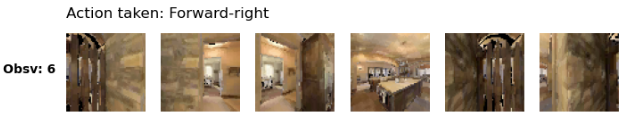
\includegraphics[scale=0.5]{figures/QUCTc6BB5sX_63289_step6.png}
        \caption{Observation taken at Steps 6 of a trajectory. The agent is hallucinating, generating text that suggests that the first image shows a kitchen sink.}
        \label{fig:fig2}
    \end{figure}
    
    In Figure \ref{fig:fig2}, the agent has identified that it is working on Navigation Checkpoint 1, which is to "\texttt{Turn your body to the left to face the sink area}"; however, it then describes Image 1 (left-most image in Figure \ref{fig:fig2}) as, "\texttt{Image 1 shows the sink area, which is the target for Navigation Checkpoint 1...}". This is an example of the how the Navigation Checkpoints list provided to the Decide Next Step module has been added to the context of the text generation and negatively influenced the image description and action decision. Such hallucinations may be a result of the limits of the smaller Qwen2-VL-7B model, and the full-size model (with 72B parameters) may not suffer from the same issues.
    \\
    \begin{figure}
        \centering
        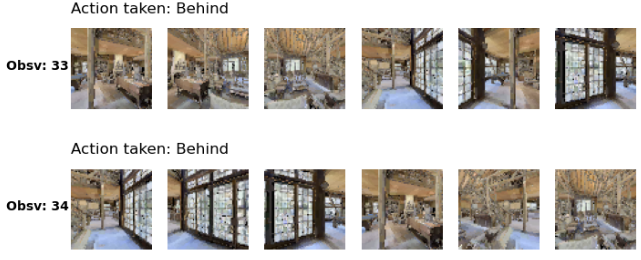
\includegraphics[scale=0.5]{figures/EU6Fwq7SyZv_16908_steps33-34.png}
        \caption{Observations taken at Steps 33 and 34 of a trajectory. The agent chooses to turn 180\textdegree a total of 10 times consecutively, switching between the observations seen in Step 33 and Step 34 and appears stuck in a cycle.}
        \label{fig:fig3}
    \end{figure}
    \\ Another example is seen in a trajectory where the agent appears stuck in a cycle. At Step 33 ("Obvs: 33") in Figure \ref{fig:fig3}, the action reasoning generated by the agent is: \\
        \texttt{I am currently working towards Navigation Checkpoint: 6 \\
        Navigation Checkpoint 6 instructions are to: Go through the open door \\
        Image that best aligns with Navigation Checkpoint 6: Image 6 shows the open door that leads to the next room, which is the next step in the instructions \\
        Selected image direction: Behind
        }
    \\ \\    
    However, the agent is mistaking Navigation Checkpoint 5 instructions (which it had already followed in Step 31)  as Navigation Checkpoint 6; furthermore, Image 6 (the right-most image in Obvs: 33) shows an image of a closed door and not an open one as the VLM suggests. Finally, Navigation Checkpoint 6 does not appear in the list of Navigation Checkpoints. In step 34 (Obvs: 34), the agent repeats most of the same reasoning, except for the final line: \\
    \texttt{Why Image 6 was selected: Image 6 shows a hallway with a rug and a door, which aligns with the instruction to go through the open door}
    \\ \\
    In this instance, the VLM is suggesting that the agent can see a hallway in Image 6 (the right-most image), despite the observation suggesting a bedroom instead. The agent then repeats the reasoning for step 33 and step 34 in a cycle for 10 steps until the stochastic nature of the VLM results in choosing the action "\texttt{Forward}" in step 43. This episode, which is repeated in other trajectories, suggests that the prompting strategies used in the modules may have further room for refinement; in particular, the Navigation History module is not conveying the context of the agent being stuck in a loop and driving more exploratory behaviour.

\section{Conclusion and Future Work}
    In this work, we developed a zero-shot small VLM-based approach to solve for the multi-modal nature of the VLN task by leveraging the vision and language capabilities of Qwen2-VL-7B. We introduced a method of generating VLN-CE training data from ground-truth data and annotations created from discrete, navigation-graph based environments, which we then used to finetune the VLM. Despite this work, it was demonstrated that the use of a single, small (7B parameter) VLM to drive a VLN agent in a continuous environment is unable to match the performance of approaches that use significantly larger models (70B+ parameters). Moving on from this work, it would be important to evaluate the performance of this approach using the Qwen2-VL-72B variant of the model to determine the performance gains from moving to a larger model. There is also significant scope for future work on refining and improving this approach. One potential area for investigation is the creation of dedicated finetuned models for each module; currently the approach described in this work uses the same VLM, which was finetuned with data relevant to all VLM modules. Investigation into adopting a discussion-based reasoning approach could also yield benefits, as demonstrated in prior work.
    Finally, the approach used in this work can be adapted easily to other models; as VLM development continues and increasingly competent models are released, there is potential for this approach to see improved performance.
    \\ \\
    \textbf{Acknowledgements}  Aside from the API being used in the this work to generate the list of Navigation Checkpoints, OpenAI's ChatGPT-4o was also used (URL: https://chatgpt.com) to assist with code debugging, trouble-shooting, and for verifying understanding of models from prior work.
    \\ I would also like to thank Dr. Altahhan and the University of Leeds for the offer of ARC4 HPC Cluster compute; whilst this work chose ultimately not to use the resource, it was useful to have this resource in reserve if other available compute became unavailable.

\printbibliography 
\end{document}